
\documentclass[final]{beamer}

\usepackage[scale=1.24]{beamerposter} % Use the beamerposter package for laying out the poster

%\usetheme{confposter} % Use the confposter theme supplied with this template
%\usetheme[faculty=chemo]{fibeamer} % Uncomment to use Masaryk University's fibeamer theme instead.

%\setbeamercolor{block title}{fg=ngreen,bg=white} % Colors of the block titles
%\setbeamercolor{block body}{fg=black,bg=white} % Colors of the body of blocks
%\setbeamercolor{block alerted title}{fg=white,bg=dblue!70} % Colors of the highlighted block titles
%\setbeamercolor{block alerted body}{fg=black,bg=dblue!10} % Colors of the body of highlighted blocks
% Many more colors are available for use in beamerthemeconfposter.sty

%-----------------------------------------------------------
% Define the column widths and overall poster size
% To set effective sepwid, onecolwid and twocolwid values, first choose how many columns you want and how much separation you want between columns
% In this template, the separation width chosen is 0.024 of the paper width and a 4-column layout
% onecolwid should therefore be (1-(# of columns+1)*sepwid)/# of columns e.g. (1-(4+1)*0.024)/4 = 0.22
% Set twocolwid to be (2*onecolwid)+sepwid = 0.464
% Set threecolwid to be (3*onecolwid)+2*sepwid = 0.708

\newlength{\sepwid}
\newlength{\onecolwid}
\newlength{\twocolwid}
\newlength{\threecolwid}
\setlength{\paperwidth}{46.8in} % A0 width: 46.8in
\setlength{\paperheight}{33.1in} % A0 height: 33.1in
\setlength{\sepwid}{0.024\paperwidth} % Separation width (white space) between columns
\setlength{\onecolwid}{0.21\paperwidth} % Width of one column
\setlength{\twocolwid}{0.451\paperwidth} % Width of two columns
\setlength{\threecolwid}{0.678\paperwidth} % Width of three columns
%\setlength{\topmargin}{-0.5in} % Reduce the top margin size
%-----------------------------------------------------------

\usepackage{graphicx}  % Required for including images

\usepackage{booktabs} % Top and bottom rules for tables

%----------------------------------------------------------------------------------------
%	TITLE SECTION 
%----------------------------------------------------------------------------------------

\usepackage{graphicx}  % Required for including images

\usepackage{booktabs} % Top and bottom rules for tables

\usepackage{here}

\usepackage[utf8]{inputenc}

\usepackage[ngerman]{babel}

\usepackage{xcolor}


\definecolor{ui-blue}{HTML}{1857c4}
\definecolor{ui-red}{HTML}{cc0012}
\setbeamercolor{block title}{fg=white,bg=ui-blue}
\setbeamercolor{block body}{fg=black,bg=}


\title{Microservices CheatSheet} % Poster title

\author{Max Jando, Joshua Vécsei} % Author(s)

\institute{Hochschule Mannheim, Fakultät für Informatik} % Institution(s)

%----------------------------------------------------------------------------------------

\begin{document}
\addtobeamertemplate{block end}{}{\vspace*{2ex}} % White space under blocks
\addtobeamertemplate{block example end}{}{\vspace*{2ex}} % White space under example blocks
\addtobeamertemplate{block alerted end}{}{\vspace*{2ex}} % White space under highlighted (alert) blocks

\setlength{\belowcaptionskip}{2ex} % White space under figures
\setlength\belowdisplayshortskip{2ex} % White space under equations
%\begin{darkframes} % Uncomment for dark theme, don't forget to \end{darkframes}
\begin{frame} % The whole poster is enclosed in one beamer frame

%==========================Begin Head===============================
  \begin{columns}
   \begin{column}{\linewidth}
    \vskip1cm
    \centering
    \usebeamercolor{title in headline}{\color{fg}\Huge{\textbf{\inserttitle}}\\[0.5ex]}
    \usebeamercolor{author in headline}{\color{fg}\Large{\insertauthor}\\[1ex]}
    \usebeamercolor{institute in headline}{\color{fg}\large{\insertinstitute}\\[1ex]}
    \vskip1cm
   \end{column}
   \vspace{1cm}
  \end{columns}
 \vspace{1cm}

%==========================End Head===============================

\begin{columns}[t] % The whole poster consists of three major columns, the second of which is split into two columns twice - the [t] option aligns each column's content to the top

\begin{column}{\sepwid}\end{column} % Empty spacer column

\begin{column}{\onecolwid} % The first column

%----------------------------------------------------------------------------------------
%	OBJECTIVES
%----------------------------------------------------------------------------------------

\begin{block}{Monolitische Hochschulanwendung}

\begin{figure}
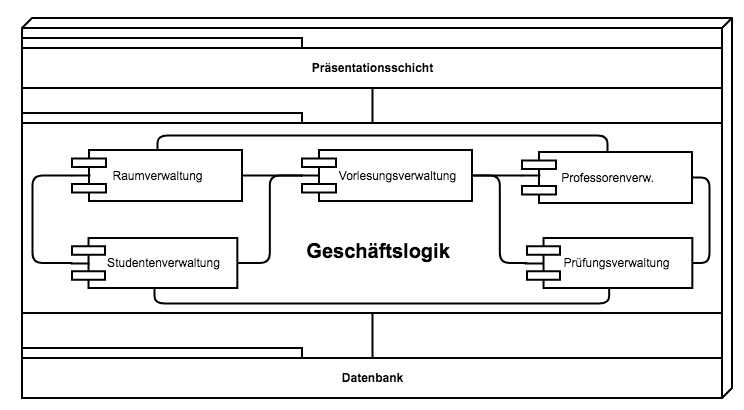
\includegraphics{monolithic_good}	
\end{figure}

\begin{itemize}
	\item Datenbank, UI und Anwendungslogik in einem
Programm - \textit{Full Stack Anwendung}
	\item Bei einem Update eine Teilkomponente muss
der ganze Monolith aktualisiert werden
	\item Nur der ganze Monolith kann skaliert werden
\item Weiterentwicklungen können unter Umständen schwer getestet werden, da die Komponenten miteinander verzahnt sind.
\end{itemize}

\end{block}

%----------------------------------------------------------------------------------------
%	INTRODUCTION
%----------------------------------------------------------------------------------------

\begin{block}{Microservices Hochschulanwendung}

\begin{figure}
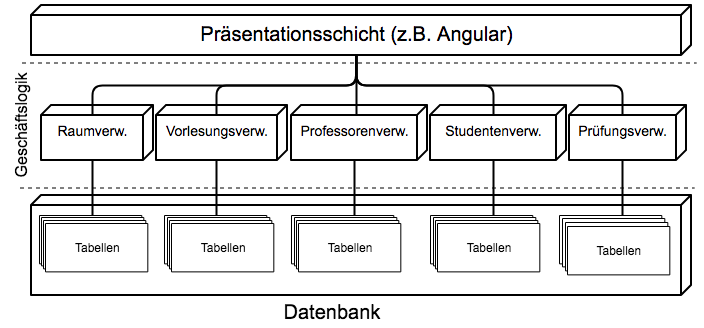
\includegraphics{microservice}	
\end{figure}

\begin{itemize}
	\item Datenbank, UI und Anwendungslogik von
einander getrennt - \textit{No Stack Anwendung}
	\item Bei einem Update einer Teilkomponente muss nur die Teilkomponente aktualisiert werden
	\item Einzelne Komponenten können gut skaliert werden
	\item Weiterentwicklungen können gut getestet werden, da die Komponenten voneinander gekoppelt sind
	\end{itemize}
\end{block}

\end{column} % End of the first column

\begin{column}{\sepwid}\end{column} % Empty spacer column

\begin{column}{\twocolwid} % Begin a column which is two columns wide (column 2)

\begin{columns}[t,totalwidth=\twocolwid] % Split up the two columns wide column

\begin{column}{\onecolwid}\vspace{-.74in} % The first column within column 2 (column 2.1)

%----------------------------------------------------------------------------------------
%	MATERIALS
%----------------------------------------------------------------------------------------

\begin{block}{Wie groß ist ein Microservice?}

\begin{figure}
	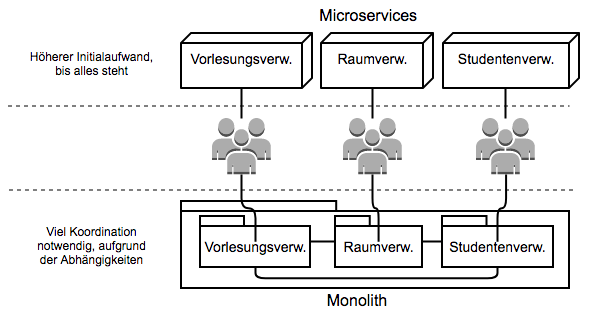
\includegraphics{teamwork}
\end{figure}

\par Unterschiedliche Faktoren spielen eine Rolle:

\begin{itemize}
	\item Teamgröße
	\item Unternehmensstruktur
	\item Abhängigkeiten der Komponenten untereinander
\end{itemize}

\begin{center}\textbf{Gefahr der Entstehung von “Nanoservices” }\end{center} 

\vspace{1cm}
\noindent

\begin{quotation}
\noindent
\begin{center}
	Erst einen Monolithen entwickeln und anschließend in Microservices aufteilen Einschätzung der Komplexität ermöglichen
\end{center}
	
\end{quotation}
\begin{center}
	(Martin Fowler)
\end{center}
\end{block}

\begin{block}{Microservice im Detail}

\begin{figure}
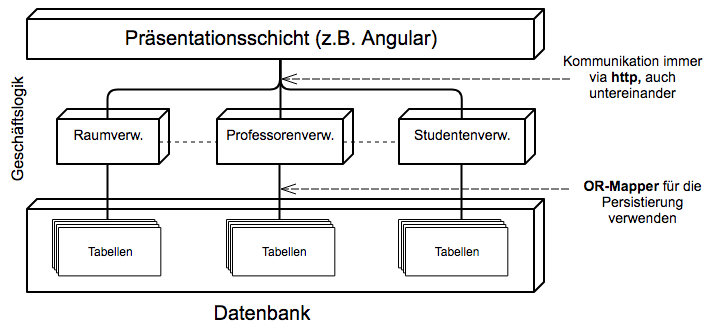
\includegraphics{microservice_detail.png}	
\end{figure}

Die Umsetzung von Microservices erfolgt i.d.R. mit einem Framework


Keine Vorgaben bezüglich der eingesetzten Technologien


REST hat sich als Architekturstil bewährt
\begin{itemize}
	\item Nutzt Standard HTTP-Methoden
	\item JSON als schlankes Austauschformat
	\item Schnittstellen sind Interoperabel
\end{itemize}

\end{block}
%----------------------------------------------------------------------------------------

\end{column} % End of column 2.1
\begin{column}{\sepwid}\end{column} % Empty spacer column

\begin{column}{\onecolwid}\vspace{-.74in} % The second column within column 2 (column 2.2)

%----------------------------------------------------------------------------------------
%	METHODS
%----------------------------------------------------------------------------------------
\begin{block}{REST Web Services}

\begin{itemize}
\item Mit  dem \textbf{RE}presentational \textbf{S}tate \textbf{T}ransfer (REST) Architekturstil lassen sich Web-Schnittstellen realisieren
\item Verwendet Standard HTTP-Methoden um CRUD-Operationen auf Ressourcen durchzuführen
\item Die vier HTTP-Verben beschreiben die durchzuführende Aktion
	\end{itemize}
	
	\begin{figure}
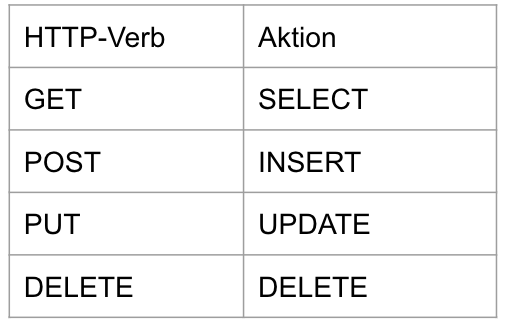
\includegraphics{http-verben}	
\end{figure}

\end{block}

\begin{block}{Welches Framework für Microservices?}

\begin{figure}
\begin{minipage}[t]{0.25\textwidth}\vspace{0pt} 

\includegraphics[width=1.0\textwidth]{spring-boot-logo} 
\end{minipage}\hfill%
\begin{minipage}[t]{0.25\textwidth}\vspace{0pt} 

\includegraphics[width=1.0\textwidth]{spark} 
\end{minipage}\hfill%
\begin{minipage}[t]{0.25\textwidth}\vspace{0pt} 

\includegraphics[width=1.0\textwidth]{vertx} 
\end{minipage}\hfill%
\end{figure}
\begin{figure}
\begin{center}
	
\includegraphics[width=0.3\textwidth]{restlet}	
\end{center}
	
\end{figure}
\par Welches Framework nun eingesetzt werden soll, ist stark abhängig davon welche Sprache man einsetzen möchte und in welcher die Entwickler am meisten Erfahrung haben. Ist die eingesetzte Sprache \textbf{Java} und persönliche Erfahrungen haben die Auswahl noch nicht weiter eingegrenzt, sollte \textbf{Spring-Boot} eingesetzt werden:

\begin{itemize}
	\item Weit verbreitetes Framework im Bereich der Java-Entwicklung
	\item Embedded-Tomcat für jeden Microservice,
	\begin{itemize}
	\item  dadurch Einfacher Start des erstellten Artefakts ohne zusätzlichen Application-Server
	\end{itemize}
	\item Schneller Einstieg möglich
	\item Gute Integration in Eclipse/IntelliJ
	\item Ausführliche Dokumentation und Tutorials zur weiteren Vertiefung im Anschluss des Workshops
\end{itemize}
	


\end{block}

%----------------------------------------------------------------------------------------

\end{column} % End of column 2.2

\end{columns} % End of the split of column 2 - any content after this will now take up 2 columns width

%----------------------------------------------------------------------------------------
%	IMPORTANT RESULT
%----------------------------------------------------------------------------------------



%----------------------------------------------------------------------------------------

\begin{columns}[t,totalwidth=\twocolwid] % Split up the two columns wide column again

\begin{column}{\onecolwid} % The first column within column 2 (column 2.1)

%----------------------------------------------------------------------------------------
%	MATHEMATICAL SECTION
%----------------------------------------------------------------------------------------


%----------------------------------------------------------------------------------------

\end{column} % End of column 2.1
\begin{column}{\sepwid}\end{column} % Empty spacer column

\begin{column}{\onecolwid} % The second column within column 2 (column 2.2)


\end{column} % End of column 2.2

\end{columns} % End of the split of column 2

\end{column} % End of the second column

\begin{column}{\sepwid}\end{column} % Empty spacer column

\begin{column}{\onecolwid} % The third column

%----------------------------------------------------------------------------------------
%	CONCLUSION
%----------------------------------------------------------------------------------------

\begin{block}{Annotationen in Spring-Boot}

Spring-Boot verwendet Annotationen um eine Microservice-Applikation zu realisieren. Nachfolgend ein Auszug einiger häufig benutzen Annotationen:

\begin{itemize}
	\item \textcolor{ui-red}{\textbf{@RestController}}: Kurzschreibweise um \textcolor{ui-red}{@Controller} und \textcolor{ui-red}{@ResponseBody} zur Klasse hinzuzufügen 
	\item \textcolor{ui-red}{\textbf{@Controller}}: Definiert die Klasse als Controller und sorgt dafür, dass Sie von Spring als solcher erkannt wird
	\item \textcolor{ui-red}{\textbf{@ResponseBody}}: Rückgabewerte von Methoden werden an die Web-Antwort angehängt
	\item \textcolor{ui-red}{\textbf{@RequestMapping}}: Weist Anfragen an den Controller (URI), den entsprechenden Methoden zu
	\item \textcolor{ui-red}{\textbf{@Autowired}}: Teilt Spring mit, dass wir ein Objekt des Typs brauchen, worüber die Annotation steht. --- \textcolor{ui-red}{@Inject} für nicht Spring-spezifisch
\item \textcolor{ui-red}{\textbf{@PostMapping / @GetMapping}}
Weist HTTP-POST / -GET Anfragen der entsprechenden Methode zu

\item \textcolor{ui-red}{\textbf{@RequestBody}}: Transformiert Informationen aus dem Body der HTTP-Anfrage in das nachstehende Objekt
\item \textcolor{ui-red}{\textbf{@SpringBootApplication}}: Notwendig damit Spring-Boot Controller und andere Komponenten finden kann. Identisch zu \textcolor{ui-red}{\textbf{@Configuration}}, \textcolor{ui-red}{\textbf{@EnableAuto Configuration}} und \textcolor{ui-red}{\textbf{@ComponentScan}}


\end{itemize}

\begin{figure}
\begin{minipage}[t]{0.40\textwidth}\vspace{0pt} 
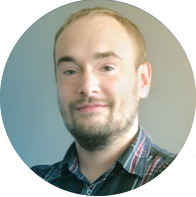
\includegraphics[width=1.0\textwidth]{maxjando} 
\begin{center}
	Max Jando
\end{center}
\end{minipage}\hfill%
\begin{minipage}[t]{0.40\textwidth}\vspace{0pt} 
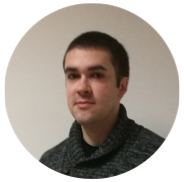
\includegraphics[width=1.0\textwidth]{joshua} 
\begin{center}
	Joshua Vécsei
\end{center}
\end{minipage}\hfill%

\end{figure}


\end{block}

%----------------------------------------------------------------------------------------

\end{column} % End of the third column

\begin{column}{\sepwid}\end{column} % Empty spacer column

\end{columns} % End of all the columns in the poster

\end{frame} % End of the enclosing frame
%\end{darkframes} % Uncomment for dark theme
\end{document}
